\section{Uncertainty and results}
Using the results of the hyperparameter search,
the final model is evaluated in more detail.
Specifically,
  the uncertainty of the predictions is analyzed, % Oxford comma
  and the physical plausibility of the predictions is investigated.


\subsection{Bootstrapping}
Bootstrapping \cite{bootstrap} is a method to estimate the uncertainty of a model.
It considers the given data as a random sample from a larger population.
Therefore,
by repeatedly sampling from the data and training a model on each sample,
the model's uncertainty can be determined
as the variance of the results of the different models.
%
For the present work, \num{50} bootstrap samples are used. % TODO
Since using a bootstrap sample of the same size as the original data set
might produce an inconsistent bootstrap estimator \cite{bootstrap_samplesize},
\num{1000000} events are used as the original data set,
while the bootstrap samples contain \num{500000} events as before.


\subsection{Energy spectrum}
\todo{
  This is (probably) the most important plot. Discuss it in more detail!
  Also: Explain percentiles etc.
}
\autoref{fig:bootstrap:distributions} shows the unfolded energy spectrum of the optimized model,
as well as the \SI{68}{\percent} confidence intervals,
  ranging from the \SI{16}{\percent} to the \SI{84}{\percent} percentile.

\blindtext[2]

\begin{figure}
  \centering
  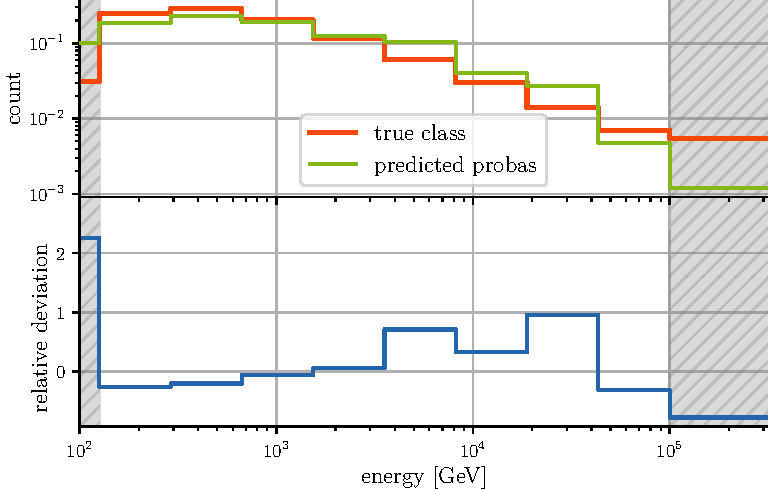
\includegraphics[scale=1]{content/plots/bootstrap:spectrum.pdf}
  \caption{
    Energy spectrum and relative deviations of the bootstrap.
    TODO: Placeholder data.
    % TODO:
    % - Add axspan to legend or explain it here.
    % - Switch to 68% confidence intervals (@Karolin)
  }
  \label{fig:bootstrap:spectrum}
\end{figure}


\subsection{Individual events}
Ordinal classification methods promise physically plausible results… % TODO
In contrast to \emph{LogisticAT},
    which \citeauthor{dsea_jan} used \cite{dsea_jan},
  the unimodality of the probability distribution is not enforced directly.
Instead,
  only the threshold probabilities ($f_k(\mathbf{x}^{[i]})$) are constrained to be monotonically increasing
  by the chain rule of probability
  (see \autoref{sec:corn:method}).
% This means that the probability distribution can be multimodal.
As can be seen in \autoref{fig:bootstrap:single_events},
  slight deviations from unimodality do occur.
  % TODO: Compare to a Random Forest?


\begin{figure}
  \centering
  % TODO: correct dimensions
  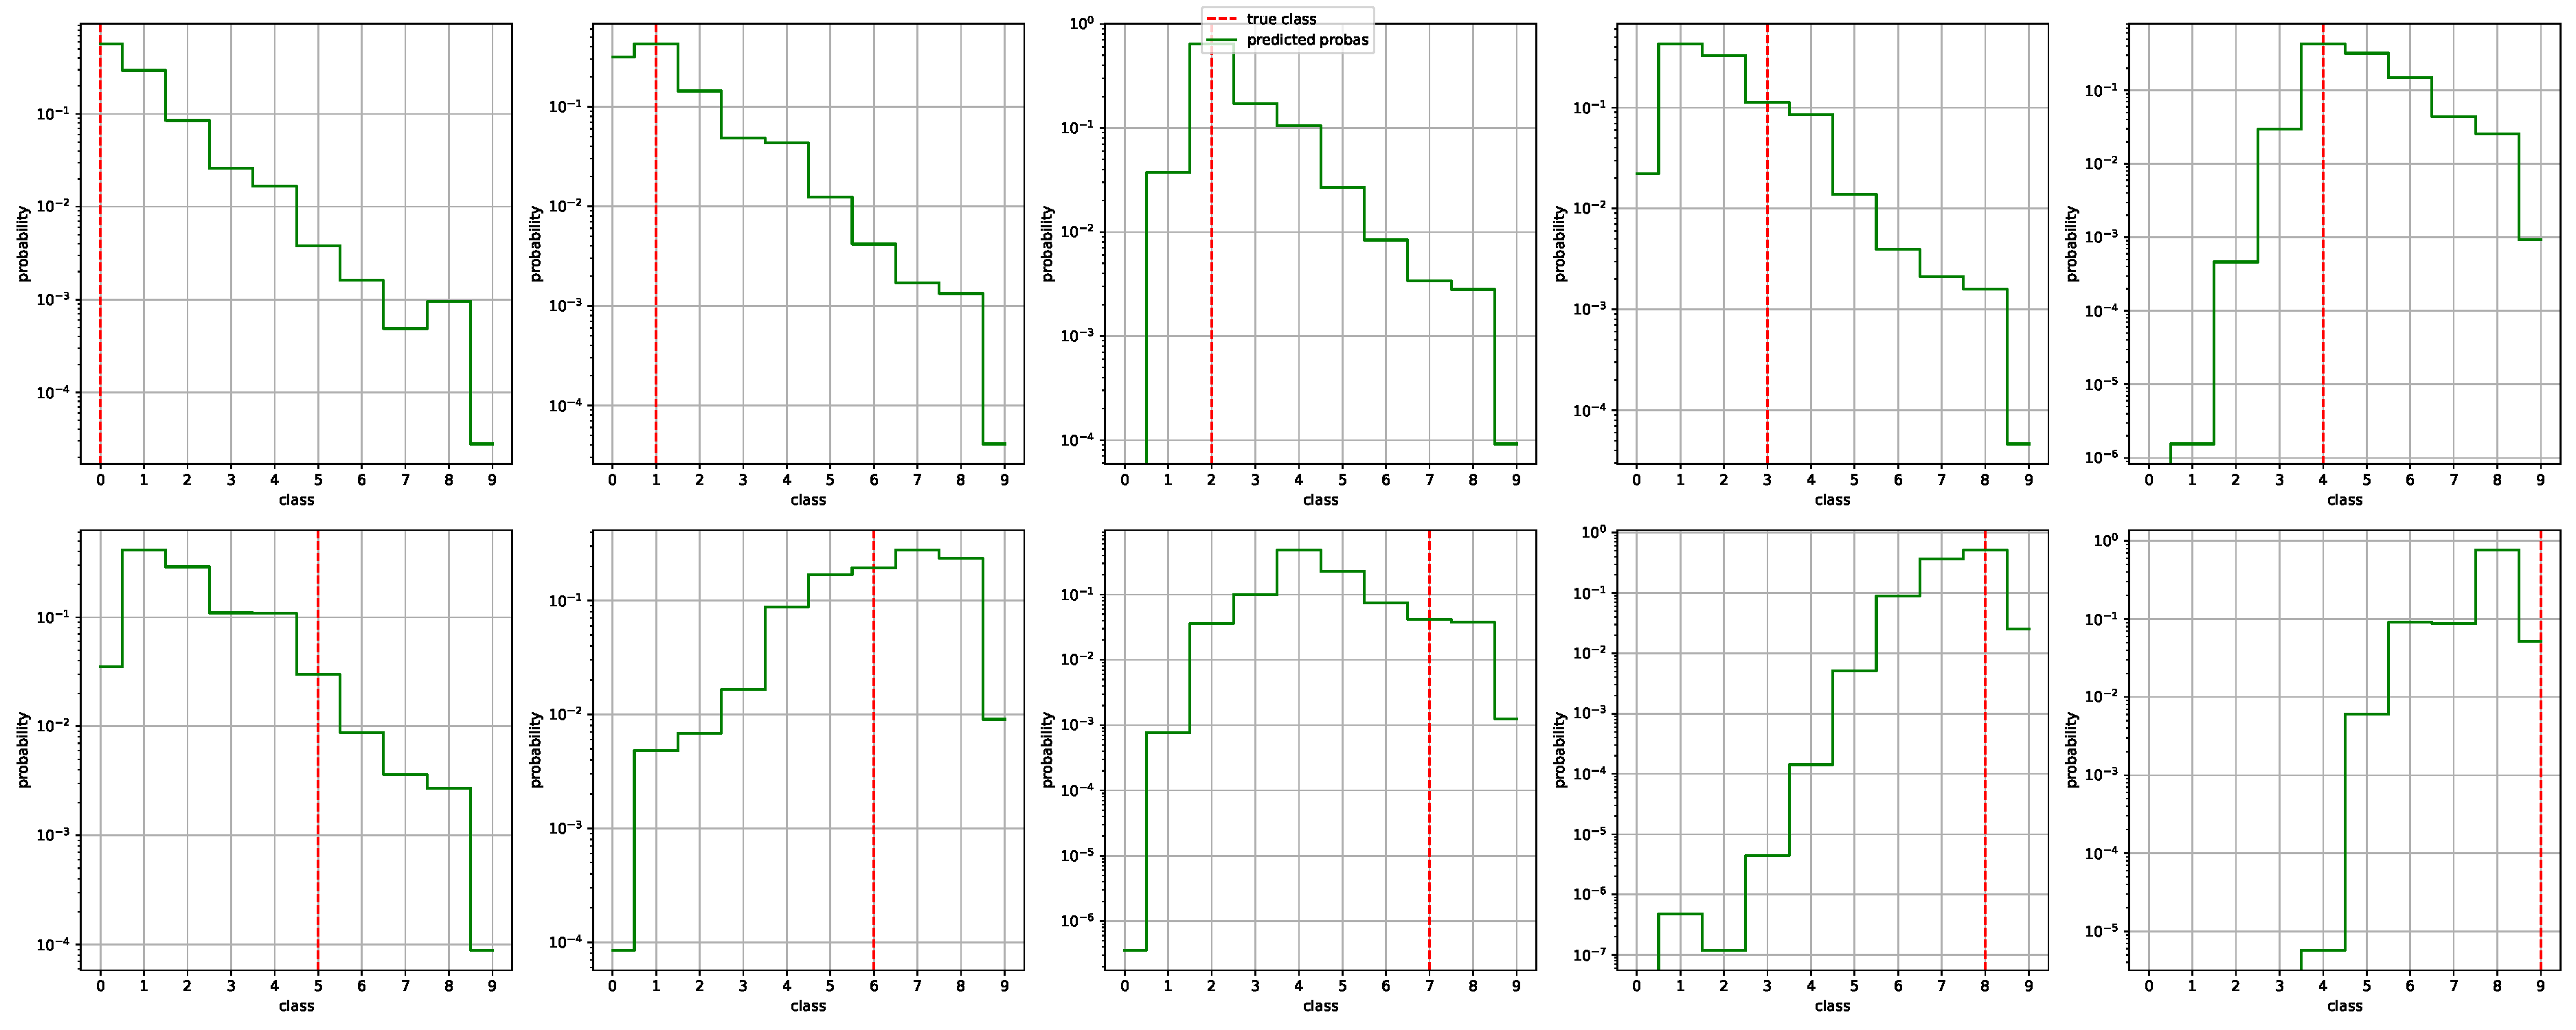
\includegraphics[width=\textwidth]{content/plots/halftime/single_events.pdf}
  \caption{
    Confidence distributions of individual events.
    For each true class,
    one random event is selected from the test set,
    and the confidence distribution of the model is shown.
  }
  \label{fig:bootstrap:single_events}
\end{figure}
